%##noBuild
\newpage
\section{Procedury}

\subsection{DOSTĘPNE MIEJSCA}
Zwraca liczbę dostępnych miejsc dla podanego id\_wycieczki.
\begin{verbatim}
CREATE OR REPLACE FUNCTION DOSTEPNE_MIEJSCA(ID_W NUMBER)
  RETURN NUMBER
IS
  LICZBA_WOLNYCH_MIEJSC NUMBER;
  BEGIN
    SELECT W.LICZBA_MIEJSC -
           NVL((SELECT COUNT(*) FROM REZERWACJE R WHERE W.ID_WYCIECZKI = R.ID_WYCIECZKI GROUP BY R.ID_WYCIECZKI),
               0) INTO LICZBA_WOLNYCH_MIEJSC
    FROM WYCIECZKI W
    WHERE W.ID_WYCIECZKI = 6;
    RETURN LICZBA_WOLNYCH_MIEJSC;
  END;
\end{verbatim}

\subsection{DODAJ REZERWACJE}
dodaj\_rezerwacje(id\_wycieczki, id\_osoby), procedura powinna kontrolować czy wycieczka
jeszcze się nie odbyła, i czy sa wolne miejsca.

\begin{verbatim}
CREATE OR REPLACE PROCEDURE DODAJ_REZERWACJE(ID_W NUMBER, ID_O NUMBER)
AS
  BEGIN
    DECLARE
      WYCIECZKI NUMBER;
      OSOBA     NUMBER;
    BEGIN

      SELECT COUNT(W.ID_WYCIECZKI) INTO WYCIECZKI FROM WYCIECZKI W WHERE W.ID_WYCIECZKI = ID_W;
      SELECT O.ID_OSOBY INTO OSOBA FROM OSOBY O WHERE O.ID_OSOBY = ID_O;

      IF WYCIECZKI > 0 AND OSOBA > 0 AND DOSTEPNE_MIEJSCA(ID_W) > 0
      THEN
        INSERT INTO REZERWACJE (ID_WYCIECZKI, ID_OSOBY, STATUS) VALUES (ID_W, ID_O, 'N');
      END IF;

    END;
  END;
\end{verbatim}\\

Po wykonaniu kodu
\begin{verbatim}
begin
  DODAJ_REZERWACJE(3, 1);
end;
\end{verbatim}
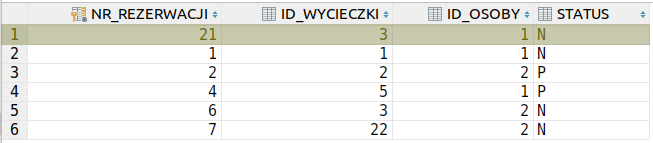
\includegraphics[width=\linewidth]{./images/dodaj_rezerwacje.png}
Pojawia się nowa rezerwacja, ponieważ wycieczka o numerze id = 3 posiada wolne miejsca oraz jej 
data rozpoczęcia jest większa od dzisiejszej daty.

\subsection{ZMIEN STATUS REZERWACJI}
zmien\_status\_rezerwacji(id\_rezerwacji, status), procedura kontrolować czy możliwa jest
zmiana statusu, np. zmiana statusu już anulowanej wycieczki (przywrócenie do stanu
aktywnego nie zawsze jest możliwe)

\begin{verbatim}
create procedure zmien_status_rezerwacji(id_rezerwacji NUMBER, nowy_status_ char)
as
  begin
    declare
      id_r            NUMBER;
      s               CHAR;
      dzisiejsza_data DATE;
    begin
      select count(r.NR_REZERWACJI) into id_r from REZERWACJE r where r.NR_REZERWACJI = id_rezerwacji;
      select r.status into s from REZERWACJE r where r.NR_REZERWACJI = id_rezerwacji;
      select current_date into dzisiejsza_data from dual;
      if id_r = 1
      then
        if (s <> 'A') and nowy_status_ in ('N', 'P', 'Z') and nowy_status_<> s
        then
          update REZERWACJE r set r.STATUS =  nowy_status_ where r.NR_REZERWACJI = id_rezerwacji;
        end if;
      end if;
    end;
  end;
\end{verbatim}

Po wykonaniu procedury:
\begin{verbatim}
begin
  ZMIEN_STATUS_REZERWACJI(7, 'P');
end;
\end{verbatim}
Następuje zmiana statusu rezerwacji dla rezerwacji o id = 7: 

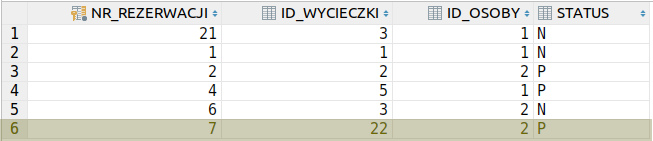
\includegraphics[width=\linewidth]{./images/zmien_status_rezerwacji.png}

\subsection{ZMIEN LICZBE MIEJSC}
zmien\_liczbe\_miejsc(id\_wycieczki, liczba\_miejsc), nie wszystkie zmiany liczby miejsc są
dozwolone, nie można zmniejszyć liczby miesc na wartość poniżej liczby zarezerwowanych
miejsc
\begin{verbatim}
CREATE OR REPLACE PROCEDURE ZMIEN_LICZBE_MIEJSC(ID_WYCIECZKI_ NUMBER, NOWA_LICZBA_MIEJSC NUMBER)
AS
  BEGIN
    DECLARE
      CALKOWITA_LICZBA_MIEJSC NUMBER;
      DOSTEPNE_MIEJSCA_ NUMBER;
    BEGIN
      SELECT W.LICZBA_MIEJSC INTO CALKOWITA_LICZBA_MIEJSC FROM WYCIECZKI W WHERE W.ID_WYCIECZKI = ID_WYCIECZKI_;
      SELECT DOSTEPNE_MIEJSCA(ID_WYCIECZKI_) INTO DOSTEPNE_MIEJSCA_ FROM DUAL;
      IF (NOWA_LICZBA_MIEJSC >= (CALKOWITA_LICZBA_MIEJSC - DOSTEPNE_MIEJSCA_))
      THEN
        UPDATE WYCIECZKI W SET W.LICZBA_MIEJSC = NOWA_LICZBA_MIEJSC WHERE W.ID_WYCIECZKI = ID_WYCIECZKI_;
      END IF;
    END;
  END;
\end{verbatim}

Po wykonaniu procedury:
\begin{verbatim}
begin
  ZMIEN_LICZBE_MIEJSC(5, 7);
end;
\end{verbatim}
Następuje zmiana miejsc dla wycieczki o id = 5:

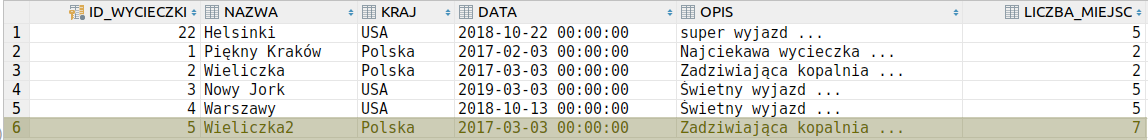
\includegraphics[width=\linewidth]{./images/zmien_liczbe_miejsc.png}
